% Options for packages loaded elsewhere
\PassOptionsToPackage{unicode}{hyperref}
\PassOptionsToPackage{hyphens}{url}
\documentclass[
  11pt,
]{article}
\usepackage{xcolor}
\usepackage[margin=1in]{geometry}
\usepackage{amsmath,amssymb}
\setcounter{secnumdepth}{5}
\usepackage{iftex}
\ifPDFTeX
  \usepackage[T1]{fontenc}
  \usepackage[utf8]{inputenc}
  \usepackage{textcomp} % provide euro and other symbols
\else % if luatex or xetex
  \usepackage{unicode-math} % this also loads fontspec
  \defaultfontfeatures{Scale=MatchLowercase}
  \defaultfontfeatures[\rmfamily]{Ligatures=TeX,Scale=1}
\fi
\usepackage{lmodern}
\ifPDFTeX\else
  % xetex/luatex font selection
\fi
% Use upquote if available, for straight quotes in verbatim environments
\IfFileExists{upquote.sty}{\usepackage{upquote}}{}
\IfFileExists{microtype.sty}{% use microtype if available
  \usepackage[]{microtype}
  \UseMicrotypeSet[protrusion]{basicmath} % disable protrusion for tt fonts
}{}
\makeatletter
\@ifundefined{KOMAClassName}{% if non-KOMA class
  \IfFileExists{parskip.sty}{%
    \usepackage{parskip}
  }{% else
    \setlength{\parindent}{0pt}
    \setlength{\parskip}{6pt plus 2pt minus 1pt}}
}{% if KOMA class
  \KOMAoptions{parskip=half}}
\makeatother
\usepackage{color}
\usepackage{fancyvrb}
\newcommand{\VerbBar}{|}
\newcommand{\VERB}{\Verb[commandchars=\\\{\}]}
\DefineVerbatimEnvironment{Highlighting}{Verbatim}{commandchars=\\\{\}}
% Add ',fontsize=\small' for more characters per line
\usepackage{framed}
\definecolor{shadecolor}{RGB}{248,248,248}
\newenvironment{Shaded}{\begin{snugshade}}{\end{snugshade}}
\newcommand{\AlertTok}[1]{\textcolor[rgb]{0.94,0.16,0.16}{#1}}
\newcommand{\AnnotationTok}[1]{\textcolor[rgb]{0.56,0.35,0.01}{\textbf{\textit{#1}}}}
\newcommand{\AttributeTok}[1]{\textcolor[rgb]{0.13,0.29,0.53}{#1}}
\newcommand{\BaseNTok}[1]{\textcolor[rgb]{0.00,0.00,0.81}{#1}}
\newcommand{\BuiltInTok}[1]{#1}
\newcommand{\CharTok}[1]{\textcolor[rgb]{0.31,0.60,0.02}{#1}}
\newcommand{\CommentTok}[1]{\textcolor[rgb]{0.56,0.35,0.01}{\textit{#1}}}
\newcommand{\CommentVarTok}[1]{\textcolor[rgb]{0.56,0.35,0.01}{\textbf{\textit{#1}}}}
\newcommand{\ConstantTok}[1]{\textcolor[rgb]{0.56,0.35,0.01}{#1}}
\newcommand{\ControlFlowTok}[1]{\textcolor[rgb]{0.13,0.29,0.53}{\textbf{#1}}}
\newcommand{\DataTypeTok}[1]{\textcolor[rgb]{0.13,0.29,0.53}{#1}}
\newcommand{\DecValTok}[1]{\textcolor[rgb]{0.00,0.00,0.81}{#1}}
\newcommand{\DocumentationTok}[1]{\textcolor[rgb]{0.56,0.35,0.01}{\textbf{\textit{#1}}}}
\newcommand{\ErrorTok}[1]{\textcolor[rgb]{0.64,0.00,0.00}{\textbf{#1}}}
\newcommand{\ExtensionTok}[1]{#1}
\newcommand{\FloatTok}[1]{\textcolor[rgb]{0.00,0.00,0.81}{#1}}
\newcommand{\FunctionTok}[1]{\textcolor[rgb]{0.13,0.29,0.53}{\textbf{#1}}}
\newcommand{\ImportTok}[1]{#1}
\newcommand{\InformationTok}[1]{\textcolor[rgb]{0.56,0.35,0.01}{\textbf{\textit{#1}}}}
\newcommand{\KeywordTok}[1]{\textcolor[rgb]{0.13,0.29,0.53}{\textbf{#1}}}
\newcommand{\NormalTok}[1]{#1}
\newcommand{\OperatorTok}[1]{\textcolor[rgb]{0.81,0.36,0.00}{\textbf{#1}}}
\newcommand{\OtherTok}[1]{\textcolor[rgb]{0.56,0.35,0.01}{#1}}
\newcommand{\PreprocessorTok}[1]{\textcolor[rgb]{0.56,0.35,0.01}{\textit{#1}}}
\newcommand{\RegionMarkerTok}[1]{#1}
\newcommand{\SpecialCharTok}[1]{\textcolor[rgb]{0.81,0.36,0.00}{\textbf{#1}}}
\newcommand{\SpecialStringTok}[1]{\textcolor[rgb]{0.31,0.60,0.02}{#1}}
\newcommand{\StringTok}[1]{\textcolor[rgb]{0.31,0.60,0.02}{#1}}
\newcommand{\VariableTok}[1]{\textcolor[rgb]{0.00,0.00,0.00}{#1}}
\newcommand{\VerbatimStringTok}[1]{\textcolor[rgb]{0.31,0.60,0.02}{#1}}
\newcommand{\WarningTok}[1]{\textcolor[rgb]{0.56,0.35,0.01}{\textbf{\textit{#1}}}}
\usepackage{graphicx}
\makeatletter
\newsavebox\pandoc@box
\newcommand*\pandocbounded[1]{% scales image to fit in text height/width
  \sbox\pandoc@box{#1}%
  \Gscale@div\@tempa{\textheight}{\dimexpr\ht\pandoc@box+\dp\pandoc@box\relax}%
  \Gscale@div\@tempb{\linewidth}{\wd\pandoc@box}%
  \ifdim\@tempb\p@<\@tempa\p@\let\@tempa\@tempb\fi% select the smaller of both
  \ifdim\@tempa\p@<\p@\scalebox{\@tempa}{\usebox\pandoc@box}%
  \else\usebox{\pandoc@box}%
  \fi%
}
% Set default figure placement to htbp
\def\fps@figure{htbp}
\makeatother
\setlength{\emergencystretch}{3em} % prevent overfull lines
\providecommand{\tightlist}{%
  \setlength{\itemsep}{0pt}\setlength{\parskip}{0pt}}
\usepackage{amsmath}
% Shared LaTeX preamble for all Data Mining / ISLR chapter documents.
% Provides \makecoverpage{<assignment title>} — a standalone title page
% with fixed student identity, so every chapter/lab looks uniform.

\usepackage{graphicx}

\newcommand{\makecoverpage}[1]{%
\begin{titlepage}
\centering
\vspace*{2cm}

{\Large \textbf{Adventist University of Central Africa}}\\[0.4cm]
{\large Master's in Big Data Analytics}\\[2cm]

{\Huge \textbf{#1}}\\[0.5cm]
{\large \textit{Introduction to Statistical Learning with Applications in R}}\\[3cm]

\begin{tabular}{rl}
\textbf{Programme:} & MSc Big Data Analytics \\
\textbf{Course Title:} & Data Mining \\
\textbf{Course Code:} & MSDA 9124 \\
\textbf{Lecturer:} & Dr. Pacifique Nizeyimana \\
\textbf{Student Name:} & Wayne Rubangisa \\
\textbf{Student ID:} & 101220 \\
\end{tabular}

\vfill

{\large September 2026}

\end{titlepage}
}

\usepackage{bookmark}
\IfFileExists{xurl.sty}{\usepackage{xurl}}{} % add URL line breaks if available
\urlstyle{same}
\hypersetup{
  hidelinks,
  pdfcreator={LaTeX via pandoc}}

\author{}
\date{\vspace{-2.5em}}

\begin{document}

\makecoverpage{Chapter 4 --- Classification \\ Lab}

\section{Introduction}\label{introduction}

Linear regression predicts a \emph{quantitative} response. But plenty of
interesting questions have a \emph{qualitative} answer instead --- will
the market go up or down today, will a customer buy the product or not,
does this email look like spam. This lab works through the main tools
for that kind of problem: logistic regression, linear and quadratic
discriminant analysis (LDA/QDA), naive Bayes, and \(K\)-nearest
neighbors, applied to three real data sets --- daily S\&P 500 returns,
caravan insurance purchases, and hourly bike-share demand.

\begin{Shaded}
\begin{Highlighting}[]
\FunctionTok{library}\NormalTok{(ISLR2)}
\FunctionTok{library}\NormalTok{(MASS)}
\FunctionTok{library}\NormalTok{(class)}
\FunctionTok{library}\NormalTok{(e1071)}
\end{Highlighting}
\end{Shaded}

\section{The Stock Market Data}\label{the-stock-market-data}

\texttt{Smarket} records the percentage return of the S\&P 500 on 1,250
trading days (2001--2005), along with the previous five days' returns
(\texttt{Lag1} through \texttt{Lag5}), trading \texttt{Volume}, and
\texttt{Direction} --- whether the market went \texttt{Up} or
\texttt{Down} that day. The question we're chasing: can
\emph{yesterday's} (and the last few days') returns predict
\emph{today's} direction at all?

\begin{Shaded}
\begin{Highlighting}[]
\FunctionTok{dim}\NormalTok{(Smarket)}
\end{Highlighting}
\end{Shaded}

\begin{verbatim}
## [1] 1250    9
\end{verbatim}

\begin{Shaded}
\begin{Highlighting}[]
\FunctionTok{summary}\NormalTok{(Smarket)}
\end{Highlighting}
\end{Shaded}

\begin{verbatim}
##       Year           Lag1                Lag2                Lag3          
##  Min.   :2001   Min.   :-4.922000   Min.   :-4.922000   Min.   :-4.922000  
##  1st Qu.:2002   1st Qu.:-0.639500   1st Qu.:-0.639500   1st Qu.:-0.640000  
##  Median :2003   Median : 0.039000   Median : 0.039000   Median : 0.038500  
##  Mean   :2003   Mean   : 0.003834   Mean   : 0.003919   Mean   : 0.001716  
##  3rd Qu.:2004   3rd Qu.: 0.596750   3rd Qu.: 0.596750   3rd Qu.: 0.596750  
##  Max.   :2005   Max.   : 5.733000   Max.   : 5.733000   Max.   : 5.733000  
##       Lag4                Lag5              Volume           Today          
##  Min.   :-4.922000   Min.   :-4.92200   Min.   :0.3561   Min.   :-4.922000  
##  1st Qu.:-0.640000   1st Qu.:-0.64000   1st Qu.:1.2574   1st Qu.:-0.639500  
##  Median : 0.038500   Median : 0.03850   Median :1.4229   Median : 0.038500  
##  Mean   : 0.001636   Mean   : 0.00561   Mean   :1.4783   Mean   : 0.003138  
##  3rd Qu.: 0.596750   3rd Qu.: 0.59700   3rd Qu.:1.6417   3rd Qu.: 0.596750  
##  Max.   : 5.733000   Max.   : 5.73300   Max.   :3.1525   Max.   : 5.733000  
##  Direction 
##  Down:602  
##  Up  :648  
##            
##            
##            
## 
\end{verbatim}

\begin{Shaded}
\begin{Highlighting}[]
\FunctionTok{cor}\NormalTok{(Smarket[, }\SpecialCharTok{{-}}\DecValTok{9}\NormalTok{])}
\end{Highlighting}
\end{Shaded}

\begin{verbatim}
##              Year         Lag1         Lag2         Lag3         Lag4
## Year   1.00000000  0.029699649  0.030596422  0.033194581  0.035688718
## Lag1   0.02969965  1.000000000 -0.026294328 -0.010803402 -0.002985911
## Lag2   0.03059642 -0.026294328  1.000000000 -0.025896670 -0.010853533
## Lag3   0.03319458 -0.010803402 -0.025896670  1.000000000 -0.024051036
## Lag4   0.03568872 -0.002985911 -0.010853533 -0.024051036  1.000000000
## Lag5   0.02978799 -0.005674606 -0.003557949 -0.018808338 -0.027083641
## Volume 0.53900647  0.040909908 -0.043383215 -0.041823686 -0.048414246
## Today  0.03009523 -0.026155045 -0.010250033 -0.002447647 -0.006899527
##                Lag5      Volume        Today
## Year    0.029787995  0.53900647  0.030095229
## Lag1   -0.005674606  0.04090991 -0.026155045
## Lag2   -0.003557949 -0.04338321 -0.010250033
## Lag3   -0.018808338 -0.04182369 -0.002447647
## Lag4   -0.027083641 -0.04841425 -0.006899527
## Lag5    1.000000000 -0.02200231 -0.034860083
## Volume -0.022002315  1.00000000  0.014591823
## Today  -0.034860083  0.01459182  1.000000000
\end{verbatim}

The correlations between the lag variables and \texttt{Today}'s return
all sit close to zero --- there's essentially no linear relationship
between recent past returns and today's. That's actually the expected,
textbook result for daily stock returns (a market that were linearly
predictable from its own recent past would be an unusually exploitable
one). The only sizable correlation in the table is between \texttt{Year}
and \texttt{Volume} --- unsurprising, since trading volume trended
upward over these five years:

\begin{Shaded}
\begin{Highlighting}[]
\FunctionTok{plot}\NormalTok{(Smarket}\SpecialCharTok{$}\NormalTok{Volume, }\AttributeTok{xlab =} \StringTok{"Chronological index"}\NormalTok{, }\AttributeTok{ylab =} \StringTok{"Volume"}\NormalTok{,}
     \AttributeTok{main =} \StringTok{"Trading volume increases over 2001{-}2005"}\NormalTok{)}
\end{Highlighting}
\end{Shaded}

\begin{center}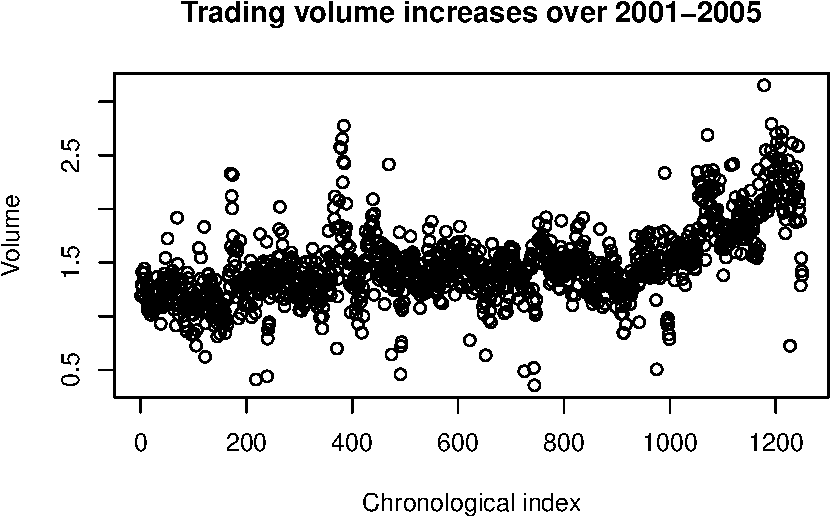
\includegraphics{ch04_lab_files/figure-latex/volume-plot-1} \end{center}

\section{Logistic Regression}\label{logistic-regression}

Since \texttt{Direction} is binary, \texttt{lm()} isn't the right tool
--- nothing stops a linear model from predicting a probability below 0
or above 1. Logistic regression instead models the probability itself
through the \emph{logistic function}, which is mathematically guaranteed
to stay in \((0,1)\) no matter what the predictors are:

\[
p(X) = P(\text{Direction = Up} \mid X) = \frac{e^{\beta_0 + \beta_1 X_1 + \cdots + \beta_p X_p}}{1 + e^{\beta_0 + \beta_1 X_1 + \cdots + \beta_p X_p}}
\]

Rearranging shows \emph{why} it's called ``logistic'' --- it's linear
not in the probability itself, but in the \textbf{log-odds}:

\[
\log\left(\frac{p(X)}{1 - p(X)}\right) = \beta_0 + \beta_1 X_1 + \cdots + \beta_p X_p
\]

So a coefficient \(\beta_j\) is read as: a one-unit increase in \(X_j\)
changes the log-odds of \texttt{Up} by \(\beta_j\), holding everything
else fixed --- not a direct change in probability, since the logistic
curve is flattest at the extremes and steepest near \(p=0.5\).

\begin{Shaded}
\begin{Highlighting}[]
\NormalTok{glm.fits }\OtherTok{\textless{}{-}} \FunctionTok{glm}\NormalTok{(}
\NormalTok{  Direction }\SpecialCharTok{\textasciitilde{}}\NormalTok{ Lag1 }\SpecialCharTok{+}\NormalTok{ Lag2 }\SpecialCharTok{+}\NormalTok{ Lag3 }\SpecialCharTok{+}\NormalTok{ Lag4 }\SpecialCharTok{+}\NormalTok{ Lag5 }\SpecialCharTok{+}\NormalTok{ Volume,}
  \AttributeTok{data =}\NormalTok{ Smarket, }\AttributeTok{family =}\NormalTok{ binomial}
\NormalTok{)}
\FunctionTok{summary}\NormalTok{(glm.fits)}
\end{Highlighting}
\end{Shaded}

\begin{verbatim}
## 
## Call:
## glm(formula = Direction ~ Lag1 + Lag2 + Lag3 + Lag4 + Lag5 + 
##     Volume, family = binomial, data = Smarket)
## 
## Coefficients:
##              Estimate Std. Error z value Pr(>|z|)
## (Intercept) -0.126000   0.240736  -0.523    0.601
## Lag1        -0.073074   0.050167  -1.457    0.145
## Lag2        -0.042301   0.050086  -0.845    0.398
## Lag3         0.011085   0.049939   0.222    0.824
## Lag4         0.009359   0.049974   0.187    0.851
## Lag5         0.010313   0.049511   0.208    0.835
## Volume       0.135441   0.158360   0.855    0.392
## 
## (Dispersion parameter for binomial family taken to be 1)
## 
##     Null deviance: 1731.2  on 1249  degrees of freedom
## Residual deviance: 1727.6  on 1243  degrees of freedom
## AIC: 1741.6
## 
## Number of Fisher Scoring iterations: 3
\end{verbatim}

None of the p-values are small --- by itself, this is a first sign that
yesterday's returns don't carry much predictive signal for today's
direction, consistent with what the correlation matrix already
suggested. \texttt{Lag1} has the smallest p-value (\(\approx 0.145\))
with a \emph{negative} coefficient, which would (weakly) suggest that a
positive return yesterday makes a positive return today slightly less
likely --- but nowhere near significant on its own.

\subsection{Confusion matrix and training
accuracy}\label{confusion-matrix-and-training-accuracy}

\begin{Shaded}
\begin{Highlighting}[]
\NormalTok{glm.probs }\OtherTok{\textless{}{-}} \FunctionTok{predict}\NormalTok{(glm.fits, }\AttributeTok{type =} \StringTok{"response"}\NormalTok{)}
\NormalTok{glm.pred }\OtherTok{\textless{}{-}} \FunctionTok{rep}\NormalTok{(}\StringTok{"Down"}\NormalTok{, }\FunctionTok{nrow}\NormalTok{(Smarket))}
\NormalTok{glm.pred[glm.probs }\SpecialCharTok{\textgreater{}} \FloatTok{0.5}\NormalTok{] }\OtherTok{\textless{}{-}} \StringTok{"Up"}

\FunctionTok{table}\NormalTok{(glm.pred, Smarket}\SpecialCharTok{$}\NormalTok{Direction)}
\end{Highlighting}
\end{Shaded}

\begin{verbatim}
##         
## glm.pred Down  Up
##     Down  145 141
##     Up    457 507
\end{verbatim}

\begin{Shaded}
\begin{Highlighting}[]
\FunctionTok{mean}\NormalTok{(glm.pred }\SpecialCharTok{==}\NormalTok{ Smarket}\SpecialCharTok{$}\NormalTok{Direction)}
\end{Highlighting}
\end{Shaded}

\begin{verbatim}
## [1] 0.5216
\end{verbatim}

About 52\% correct --- barely better than a coin flip, and misleadingly
so: this is \textbf{training} accuracy, computed on the exact data the
model was fit to. A model that just memorizes noise in the training set
can look fine here and still fail on new data --- which is exactly why
we need a genuine held-out test set.

\subsection{A real train/test split}\label{a-real-traintest-split}

We use the classic ``hold out the future'' split for time series data:
train on 2001--2004, and test on 2005 --- data the model has never seen.

\begin{Shaded}
\begin{Highlighting}[]
\NormalTok{train }\OtherTok{\textless{}{-}}\NormalTok{ Smarket}\SpecialCharTok{$}\NormalTok{Year }\SpecialCharTok{\textless{}} \DecValTok{2005}
\NormalTok{Smarket}\FloatTok{.2005} \OtherTok{\textless{}{-}}\NormalTok{ Smarket[}\SpecialCharTok{!}\NormalTok{train, ]}
\NormalTok{Direction}\FloatTok{.2005} \OtherTok{\textless{}{-}}\NormalTok{ Smarket}\SpecialCharTok{$}\NormalTok{Direction[}\SpecialCharTok{!}\NormalTok{train]}
\FunctionTok{dim}\NormalTok{(Smarket}\FloatTok{.2005}\NormalTok{)}
\end{Highlighting}
\end{Shaded}

\begin{verbatim}
## [1] 252   9
\end{verbatim}

\begin{Shaded}
\begin{Highlighting}[]
\NormalTok{glm.fits }\OtherTok{\textless{}{-}} \FunctionTok{glm}\NormalTok{(}
\NormalTok{  Direction }\SpecialCharTok{\textasciitilde{}}\NormalTok{ Lag1 }\SpecialCharTok{+}\NormalTok{ Lag2 }\SpecialCharTok{+}\NormalTok{ Lag3 }\SpecialCharTok{+}\NormalTok{ Lag4 }\SpecialCharTok{+}\NormalTok{ Lag5 }\SpecialCharTok{+}\NormalTok{ Volume,}
  \AttributeTok{data =}\NormalTok{ Smarket, }\AttributeTok{family =}\NormalTok{ binomial, }\AttributeTok{subset =}\NormalTok{ train}
\NormalTok{)}
\NormalTok{glm.probs }\OtherTok{\textless{}{-}} \FunctionTok{predict}\NormalTok{(glm.fits, Smarket}\FloatTok{.2005}\NormalTok{, }\AttributeTok{type =} \StringTok{"response"}\NormalTok{)}
\NormalTok{glm.pred }\OtherTok{\textless{}{-}} \FunctionTok{rep}\NormalTok{(}\StringTok{"Down"}\NormalTok{, }\FunctionTok{nrow}\NormalTok{(Smarket}\FloatTok{.2005}\NormalTok{))}
\NormalTok{glm.pred[glm.probs }\SpecialCharTok{\textgreater{}} \FloatTok{0.5}\NormalTok{] }\OtherTok{\textless{}{-}} \StringTok{"Up"}

\FunctionTok{table}\NormalTok{(glm.pred, Direction}\FloatTok{.2005}\NormalTok{)}
\end{Highlighting}
\end{Shaded}

\begin{verbatim}
##         Direction.2005
## glm.pred Down Up
##     Down   77 97
##     Up     34 44
\end{verbatim}

\begin{Shaded}
\begin{Highlighting}[]
\FunctionTok{mean}\NormalTok{(glm.pred }\SpecialCharTok{==}\NormalTok{ Direction}\FloatTok{.2005}\NormalTok{)}
\end{Highlighting}
\end{Shaded}

\begin{verbatim}
## [1] 0.4801587
\end{verbatim}

Test accuracy is \emph{worse} than training accuracy here --- actually
worse than just always guessing \texttt{Up}, which is a sign the full
five-lag model is overfitting noise rather than finding real signal.
Since \texttt{Lag1} and \texttt{Lag2} were the two most promising
predictors above, it's worth trying a leaner model:

\begin{Shaded}
\begin{Highlighting}[]
\NormalTok{glm.fits }\OtherTok{\textless{}{-}} \FunctionTok{glm}\NormalTok{(Direction }\SpecialCharTok{\textasciitilde{}}\NormalTok{ Lag1 }\SpecialCharTok{+}\NormalTok{ Lag2, }\AttributeTok{data =}\NormalTok{ Smarket,}
                 \AttributeTok{family =}\NormalTok{ binomial, }\AttributeTok{subset =}\NormalTok{ train)}
\NormalTok{glm.probs }\OtherTok{\textless{}{-}} \FunctionTok{predict}\NormalTok{(glm.fits, Smarket}\FloatTok{.2005}\NormalTok{, }\AttributeTok{type =} \StringTok{"response"}\NormalTok{)}
\NormalTok{glm.pred }\OtherTok{\textless{}{-}} \FunctionTok{rep}\NormalTok{(}\StringTok{"Down"}\NormalTok{, }\FunctionTok{nrow}\NormalTok{(Smarket}\FloatTok{.2005}\NormalTok{))}
\NormalTok{glm.pred[glm.probs }\SpecialCharTok{\textgreater{}} \FloatTok{0.5}\NormalTok{] }\OtherTok{\textless{}{-}} \StringTok{"Up"}

\FunctionTok{table}\NormalTok{(glm.pred, Direction}\FloatTok{.2005}\NormalTok{)}
\end{Highlighting}
\end{Shaded}

\begin{verbatim}
##         Direction.2005
## glm.pred Down  Up
##     Down   35  35
##     Up     76 106
\end{verbatim}

\begin{Shaded}
\begin{Highlighting}[]
\FunctionTok{mean}\NormalTok{(glm.pred }\SpecialCharTok{==}\NormalTok{ Direction}\FloatTok{.2005}\NormalTok{)}
\end{Highlighting}
\end{Shaded}

\begin{verbatim}
## [1] 0.5595238
\end{verbatim}

That's a meaningful improvement --- dropping the three weakest
predictors actually helped test performance, a concrete illustration of
the bias-variance idea from Chapter 2: a model with fewer, better-chosen
predictors can generalize better than one that includes everything, even
though it necessarily has strictly worse (or equal) training fit.

\section{Linear Discriminant
Analysis}\label{linear-discriminant-analysis}

Logistic regression models \(P(Y \mid X)\) directly. LDA takes the
opposite route --- Bayes' theorem in reverse --- modeling how \(X\) is
distributed \emph{within} each class, then using Bayes' rule to get back
to \(P(Y \mid X)\):

\[
P(Y = k \mid X = x) = \frac{\pi_k \, f_k(x)}{\sum_{l} \pi_l \, f_l(x)}
\]

where \(\pi_k\) is the (estimated) prior probability of class \(k\), and
\(f_k(x)\) is the density of \(X\) within class \(k\). LDA's specific
assumption is that each class's predictors follow a Gaussian
distribution, all sharing the \emph{same} covariance structure --- only
the class means differ. Under that assumption the decision boundary
between classes works out to be linear, which is where LDA gets its
name.

\begin{Shaded}
\begin{Highlighting}[]
\NormalTok{lda.fit }\OtherTok{\textless{}{-}} \FunctionTok{lda}\NormalTok{(Direction }\SpecialCharTok{\textasciitilde{}}\NormalTok{ Lag1 }\SpecialCharTok{+}\NormalTok{ Lag2, }\AttributeTok{data =}\NormalTok{ Smarket, }\AttributeTok{subset =}\NormalTok{ train)}
\NormalTok{lda.fit}
\end{Highlighting}
\end{Shaded}

\begin{verbatim}
## Call:
## lda(Direction ~ Lag1 + Lag2, data = Smarket, subset = train)
## 
## Prior probabilities of groups:
##     Down       Up 
## 0.491984 0.508016 
## 
## Group means:
##             Lag1        Lag2
## Down  0.04279022  0.03389409
## Up   -0.03954635 -0.03132544
## 
## Coefficients of linear discriminants:
##             LD1
## Lag1 -0.6420190
## Lag2 -0.5135293
\end{verbatim}

The \textbf{prior probabilities}
(\(\hat\pi_{\text{Down}} \approx 0.492\),
\(\hat\pi_{\text{Up}} \approx 0.508\)) are just the class proportions in
the training data. The \textbf{group means} show that on \texttt{Up}
days, \texttt{Lag1} and \texttt{Lag2} tend to be slightly negative on
average --- consistent with the (weak) negative association logistic
regression also picked up.

\begin{Shaded}
\begin{Highlighting}[]
\NormalTok{lda.pred }\OtherTok{\textless{}{-}} \FunctionTok{predict}\NormalTok{(lda.fit, Smarket}\FloatTok{.2005}\NormalTok{)}
\FunctionTok{table}\NormalTok{(lda.pred}\SpecialCharTok{$}\NormalTok{class, Direction}\FloatTok{.2005}\NormalTok{)}
\end{Highlighting}
\end{Shaded}

\begin{verbatim}
##       Direction.2005
##        Down  Up
##   Down   35  35
##   Up     76 106
\end{verbatim}

\begin{Shaded}
\begin{Highlighting}[]
\FunctionTok{mean}\NormalTok{(lda.pred}\SpecialCharTok{$}\NormalTok{class }\SpecialCharTok{==}\NormalTok{ Direction}\FloatTok{.2005}\NormalTok{)}
\end{Highlighting}
\end{Shaded}

\begin{verbatim}
## [1] 0.5595238
\end{verbatim}

Almost identical accuracy to the leaner logistic regression --- not a
coincidence. With two classes and (roughly) Gaussian, similarly-shaped
predictors, LDA and logistic regression tend to land on very similar
decision boundaries, even though they get there through different routes
(generative vs.~discriminative modeling).

\section{Quadratic Discriminant
Analysis}\label{quadratic-discriminant-analysis}

QDA relaxes LDA's shared-covariance assumption --- each class gets its
\emph{own} covariance matrix. That extra flexibility means the decision
boundary is now quadratic rather than linear, at the cost of estimating
more parameters (and so needing more data to do it reliably).

\begin{Shaded}
\begin{Highlighting}[]
\NormalTok{qda.fit }\OtherTok{\textless{}{-}} \FunctionTok{qda}\NormalTok{(Direction }\SpecialCharTok{\textasciitilde{}}\NormalTok{ Lag1 }\SpecialCharTok{+}\NormalTok{ Lag2, }\AttributeTok{data =}\NormalTok{ Smarket, }\AttributeTok{subset =}\NormalTok{ train)}
\NormalTok{qda.fit}
\end{Highlighting}
\end{Shaded}

\begin{verbatim}
## Call:
## qda(Direction ~ Lag1 + Lag2, data = Smarket, subset = train)
## 
## Prior probabilities of groups:
##     Down       Up 
## 0.491984 0.508016 
## 
## Group means:
##             Lag1        Lag2
## Down  0.04279022  0.03389409
## Up   -0.03954635 -0.03132544
\end{verbatim}

\begin{Shaded}
\begin{Highlighting}[]
\NormalTok{qda.class }\OtherTok{\textless{}{-}} \FunctionTok{predict}\NormalTok{(qda.fit, Smarket}\FloatTok{.2005}\NormalTok{)}\SpecialCharTok{$}\NormalTok{class}
\FunctionTok{table}\NormalTok{(qda.class, Direction}\FloatTok{.2005}\NormalTok{)}
\end{Highlighting}
\end{Shaded}

\begin{verbatim}
##          Direction.2005
## qda.class Down  Up
##      Down   30  20
##      Up     81 121
\end{verbatim}

\begin{Shaded}
\begin{Highlighting}[]
\FunctionTok{mean}\NormalTok{(qda.class }\SpecialCharTok{==}\NormalTok{ Direction}\FloatTok{.2005}\NormalTok{)}
\end{Highlighting}
\end{Shaded}

\begin{verbatim}
## [1] 0.5992063
\end{verbatim}

QDA edges out both logistic regression and LDA here. One reading: the
true boundary between \texttt{Up} and \texttt{Down} days may genuinely
be closer to quadratic than linear --- but with only two predictors and
a few hundred test observations, this could also just be QDA getting
fortunate on this particular test split rather than a guaranteed
generalizable edge.

\section{Naive Bayes}\label{naive-bayes}

Naive Bayes keeps the same generative Bayes'-rule structure as LDA/QDA,
but replaces the Gaussian-with-shared/class-specific-covariance
assumption with something blunter and computationally cheaper: it
assumes every predictor is \textbf{independent of every other predictor,
within each class}.

\[
f_k(x) = f_{k1}(x_1) \times f_{k2}(x_2) \times \cdots \times f_{kp}(x_p)
\]

This is rarely \emph{exactly} true --- \texttt{Lag1} and \texttt{Lag2}
are unlikely to be truly independent given \texttt{Direction} --- but it
collapses a hard multivariate density-estimation problem into \(p\) easy
univariate ones, and in practice often still classifies well even when
the independence assumption is technically wrong.

\begin{Shaded}
\begin{Highlighting}[]
\NormalTok{nb.fit }\OtherTok{\textless{}{-}} \FunctionTok{naiveBayes}\NormalTok{(Direction }\SpecialCharTok{\textasciitilde{}}\NormalTok{ Lag1 }\SpecialCharTok{+}\NormalTok{ Lag2, }\AttributeTok{data =}\NormalTok{ Smarket, }\AttributeTok{subset =}\NormalTok{ train)}
\NormalTok{nb.fit}
\end{Highlighting}
\end{Shaded}

\begin{verbatim}
## 
## Naive Bayes Classifier for Discrete Predictors
## 
## Call:
## naiveBayes.default(x = X, y = Y, laplace = laplace)
## 
## A-priori probabilities:
## Y
##     Down       Up 
## 0.491984 0.508016 
## 
## Conditional probabilities:
##       Lag1
## Y             [,1]     [,2]
##   Down  0.04279022 1.227446
##   Up   -0.03954635 1.231668
## 
##       Lag2
## Y             [,1]     [,2]
##   Down  0.03389409 1.239191
##   Up   -0.03132544 1.220765
\end{verbatim}

\begin{Shaded}
\begin{Highlighting}[]
\NormalTok{nb.class }\OtherTok{\textless{}{-}} \FunctionTok{predict}\NormalTok{(nb.fit, Smarket}\FloatTok{.2005}\NormalTok{)}
\FunctionTok{table}\NormalTok{(nb.class, Direction}\FloatTok{.2005}\NormalTok{)}
\end{Highlighting}
\end{Shaded}

\begin{verbatim}
##         Direction.2005
## nb.class Down  Up
##     Down   28  20
##     Up     83 121
\end{verbatim}

\begin{Shaded}
\begin{Highlighting}[]
\FunctionTok{mean}\NormalTok{(nb.class }\SpecialCharTok{==}\NormalTok{ Direction}\FloatTok{.2005}\NormalTok{)}
\end{Highlighting}
\end{Shaded}

\begin{verbatim}
## [1] 0.5912698
\end{verbatim}

Performance here lands close to LDA and logistic regression ---
reasonable, since with only two predictors there's less room for the
independence assumption to cause real damage than there would be with
many correlated predictors.

\section{\texorpdfstring{\(K\)-Nearest
Neighbors}{K-Nearest Neighbors}}\label{k-nearest-neighbors}

Every method so far assumes some parametric form for how
\texttt{Direction} depends on the predictors (a linear log-odds, a
Gaussian density, \ldots). KNN assumes nothing about the shape of the
boundary at all: to classify a new point, find its \(K\) nearest
neighbors in the training data (by Euclidean distance) and take a
majority vote among them.

\begin{Shaded}
\begin{Highlighting}[]
\NormalTok{train.X }\OtherTok{\textless{}{-}} \FunctionTok{cbind}\NormalTok{(Smarket}\SpecialCharTok{$}\NormalTok{Lag1, Smarket}\SpecialCharTok{$}\NormalTok{Lag2)[train, ]}
\NormalTok{test.X }\OtherTok{\textless{}{-}} \FunctionTok{cbind}\NormalTok{(Smarket}\SpecialCharTok{$}\NormalTok{Lag1, Smarket}\SpecialCharTok{$}\NormalTok{Lag2)[}\SpecialCharTok{!}\NormalTok{train, ]}
\NormalTok{train.Direction }\OtherTok{\textless{}{-}}\NormalTok{ Smarket}\SpecialCharTok{$}\NormalTok{Direction[train]}

\FunctionTok{set.seed}\NormalTok{(}\DecValTok{1}\NormalTok{)}
\NormalTok{knn.pred }\OtherTok{\textless{}{-}} \FunctionTok{knn}\NormalTok{(train.X, test.X, train.Direction, }\AttributeTok{k =} \DecValTok{1}\NormalTok{)}
\FunctionTok{table}\NormalTok{(knn.pred, Direction}\FloatTok{.2005}\NormalTok{)}
\end{Highlighting}
\end{Shaded}

\begin{verbatim}
##         Direction.2005
## knn.pred Down Up
##     Down   43 58
##     Up     68 83
\end{verbatim}

\begin{Shaded}
\begin{Highlighting}[]
\FunctionTok{mean}\NormalTok{(knn.pred }\SpecialCharTok{==}\NormalTok{ Direction}\FloatTok{.2005}\NormalTok{)}
\end{Highlighting}
\end{Shaded}

\begin{verbatim}
## [1] 0.5
\end{verbatim}

\(K=1\) is the most flexible possible choice --- each test point is
classified by whichever single training point happens to be closest,
which chases noise aggressively and shows in the roughly 50\% accuracy
(no better than guessing). Bumping \(K\) up trades away some of that
flexibility for stability:

\begin{Shaded}
\begin{Highlighting}[]
\NormalTok{knn.pred }\OtherTok{\textless{}{-}} \FunctionTok{knn}\NormalTok{(train.X, test.X, train.Direction, }\AttributeTok{k =} \DecValTok{3}\NormalTok{)}
\FunctionTok{table}\NormalTok{(knn.pred, Direction}\FloatTok{.2005}\NormalTok{)}
\end{Highlighting}
\end{Shaded}

\begin{verbatim}
##         Direction.2005
## knn.pred Down Up
##     Down   48 54
##     Up     63 87
\end{verbatim}

\begin{Shaded}
\begin{Highlighting}[]
\FunctionTok{mean}\NormalTok{(knn.pred }\SpecialCharTok{==}\NormalTok{ Direction}\FloatTok{.2005}\NormalTok{)}
\end{Highlighting}
\end{Shaded}

\begin{verbatim}
## [1] 0.5357143
\end{verbatim}

A modest improvement, but still well short of QDA. Altogether, across
every method tried, \texttt{Lag1}/\texttt{Lag2} simply don't carry much
signal about \texttt{Direction} --- which, again, is the expected
finding for daily stock returns, not a failure of the methods
themselves.

\subsection{Application: Caravan
Insurance}\label{application-caravan-insurance}

\texttt{Caravan} is a more favorable setting for KNN: 5,822 customers,
85 demographic predictors, and a binary \texttt{Purchase} outcome (did
they buy caravan insurance). Because KNN measures raw Euclidean
distance, any predictor on a larger numeric scale automatically
dominates the distance calculation regardless of how informative it
actually is --- so predictors need to be standardized first:

\begin{Shaded}
\begin{Highlighting}[]
\NormalTok{standardized.X }\OtherTok{\textless{}{-}} \FunctionTok{scale}\NormalTok{(Caravan[, }\SpecialCharTok{{-}}\DecValTok{86}\NormalTok{])}
\FunctionTok{mean}\NormalTok{(Caravan[[}\DecValTok{1}\NormalTok{]]); }\FunctionTok{mean}\NormalTok{(Caravan[[}\DecValTok{2}\NormalTok{]])}
\end{Highlighting}
\end{Shaded}

\begin{verbatim}
## [1] 24.25335
\end{verbatim}

\begin{verbatim}
## [1] 1.110615
\end{verbatim}

\begin{Shaded}
\begin{Highlighting}[]
\FunctionTok{var}\NormalTok{(standardized.X[, }\DecValTok{1}\NormalTok{]); }\FunctionTok{var}\NormalTok{(standardized.X[, }\DecValTok{2}\NormalTok{])}
\end{Highlighting}
\end{Shaded}

\begin{verbatim}
## [1] 1
\end{verbatim}

\begin{verbatim}
## [1] 1
\end{verbatim}

After scaling, every predictor has variance 1, so no single variable can
dominate the distance metric purely because of its units.

\begin{Shaded}
\begin{Highlighting}[]
\NormalTok{test }\OtherTok{\textless{}{-}} \DecValTok{1}\SpecialCharTok{:}\DecValTok{1000}
\NormalTok{train.X }\OtherTok{\textless{}{-}}\NormalTok{ standardized.X[}\SpecialCharTok{{-}}\NormalTok{test, ]}
\NormalTok{test.X }\OtherTok{\textless{}{-}}\NormalTok{ standardized.X[test, ]}
\NormalTok{train.Y }\OtherTok{\textless{}{-}}\NormalTok{ Caravan}\SpecialCharTok{$}\NormalTok{Purchase[}\SpecialCharTok{{-}}\NormalTok{test]}
\NormalTok{test.Y }\OtherTok{\textless{}{-}}\NormalTok{ Caravan}\SpecialCharTok{$}\NormalTok{Purchase[test]}

\FunctionTok{set.seed}\NormalTok{(}\DecValTok{1}\NormalTok{)}
\NormalTok{knn.pred }\OtherTok{\textless{}{-}} \FunctionTok{knn}\NormalTok{(train.X, test.X, train.Y, }\AttributeTok{k =} \DecValTok{3}\NormalTok{)}
\FunctionTok{table}\NormalTok{(knn.pred, test.Y)}
\end{Highlighting}
\end{Shaded}

\begin{verbatim}
##         test.Y
## knn.pred  No Yes
##      No  921  54
##      Yes  20   5
\end{verbatim}

Only about 6\% of customers actually purchase, so overall accuracy is a
misleading metric here --- a model that always predicts ``No'' would
already be right about 94\% of the time. What actually matters for a
marketing campaign is \emph{precision among predicted buyers}: of the
customers KNN flagged as likely purchasers, what fraction really did
buy? That's a meaningfully higher hit rate than the 6\% baseline rate,
which is the actual value of the model --- it concentrates marketing
spend on customers substantially more likely to convert than a random
customer would be.

\section{Poisson Regression}\label{poisson-regression}

\texttt{Bikeshare} records hourly bike rental counts (\texttt{bikers})
along with weather and calendar predictors. A count that's always
\(\geq 0\) and often small doesn't fit the assumptions of ordinary
linear regression well --- a linear model can happily predict a negative
number of bike rentals, which is nonsensical. Poisson regression is
built for exactly this: it assumes
\(Y \mid X \sim \text{Poisson}(\lambda(X))\), and --- just like logistic
regression links probability through the logistic function --- links the
rate \(\lambda\) through a \textbf{log} link, guaranteeing predictions
stay positive:

\[
\log(\lambda(X)) = \beta_0 + \beta_1 X_1 + \cdots + \beta_p X_p
\qquad \Longleftrightarrow \qquad
\lambda(X) = e^{\beta_0 + \beta_1 X_1 + \cdots + \beta_p X_p}
\]

A coefficient \(\beta_j\) is therefore read multiplicatively: a one-unit
increase in \(X_j\) multiplies the expected count by \(e^{\beta_j}\),
holding other predictors fixed.

\begin{Shaded}
\begin{Highlighting}[]
\NormalTok{mod.pois }\OtherTok{\textless{}{-}} \FunctionTok{glm}\NormalTok{(}
\NormalTok{  bikers }\SpecialCharTok{\textasciitilde{}}\NormalTok{ mnth }\SpecialCharTok{+}\NormalTok{ hr }\SpecialCharTok{+}\NormalTok{ workingday }\SpecialCharTok{+}\NormalTok{ temp }\SpecialCharTok{+}\NormalTok{ weathersit,}
  \AttributeTok{data =}\NormalTok{ Bikeshare, }\AttributeTok{family =}\NormalTok{ poisson}
\NormalTok{)}
\FunctionTok{summary}\NormalTok{(mod.pois)}
\end{Highlighting}
\end{Shaded}

\begin{verbatim}
## 
## Call:
## glm(formula = bikers ~ mnth + hr + workingday + temp + weathersit, 
##     family = poisson, data = Bikeshare)
## 
## Coefficients:
##                            Estimate Std. Error  z value Pr(>|z|)    
## (Intercept)                2.693688   0.009720  277.124  < 2e-16 ***
## mnthFeb                    0.226046   0.006951   32.521  < 2e-16 ***
## mnthMarch                  0.376437   0.006691   56.263  < 2e-16 ***
## mnthApril                  0.691693   0.006987   98.996  < 2e-16 ***
## mnthMay                    0.910641   0.007436  122.469  < 2e-16 ***
## mnthJune                   0.893405   0.008242  108.402  < 2e-16 ***
## mnthJuly                   0.773787   0.008806   87.874  < 2e-16 ***
## mnthAug                    0.821341   0.008332   98.573  < 2e-16 ***
## mnthSept                   0.903663   0.007621  118.578  < 2e-16 ***
## mnthOct                    0.937743   0.006744  139.054  < 2e-16 ***
## mnthNov                    0.820433   0.006494  126.334  < 2e-16 ***
## mnthDec                    0.686850   0.006317  108.724  < 2e-16 ***
## hr1                       -0.471593   0.012999  -36.278  < 2e-16 ***
## hr2                       -0.808761   0.014646  -55.220  < 2e-16 ***
## hr3                       -1.443918   0.018843  -76.631  < 2e-16 ***
## hr4                       -2.076098   0.024796  -83.728  < 2e-16 ***
## hr5                       -1.060271   0.016075  -65.957  < 2e-16 ***
## hr6                        0.324498   0.010610   30.585  < 2e-16 ***
## hr7                        1.329567   0.009056  146.822  < 2e-16 ***
## hr8                        1.831313   0.008653  211.630  < 2e-16 ***
## hr9                        1.336155   0.009016  148.191  < 2e-16 ***
## hr10                       1.091238   0.009261  117.831  < 2e-16 ***
## hr11                       1.248507   0.009093  137.304  < 2e-16 ***
## hr12                       1.434028   0.008936  160.486  < 2e-16 ***
## hr13                       1.427951   0.008951  159.529  < 2e-16 ***
## hr14                       1.379296   0.008999  153.266  < 2e-16 ***
## hr15                       1.408149   0.008977  156.862  < 2e-16 ***
## hr16                       1.628688   0.008805  184.979  < 2e-16 ***
## hr17                       2.049021   0.008565  239.221  < 2e-16 ***
## hr18                       1.966668   0.008586  229.065  < 2e-16 ***
## hr19                       1.668409   0.008743  190.830  < 2e-16 ***
## hr20                       1.370588   0.008973  152.737  < 2e-16 ***
## hr21                       1.118568   0.009215  121.383  < 2e-16 ***
## hr22                       0.871879   0.009536   91.429  < 2e-16 ***
## hr23                       0.481387   0.010207   47.164  < 2e-16 ***
## workingday                 0.014665   0.001955    7.502 6.27e-14 ***
## temp                       0.785292   0.011475   68.434  < 2e-16 ***
## weathersitcloudy/misty    -0.075231   0.002179  -34.528  < 2e-16 ***
## weathersitlight rain/snow -0.575800   0.004058 -141.905  < 2e-16 ***
## weathersitheavy rain/snow -0.926287   0.166782   -5.554 2.79e-08 ***
## ---
## Signif. codes:  0 '***' 0.001 '**' 0.01 '*' 0.05 '.' 0.1 ' ' 1
## 
## (Dispersion parameter for poisson family taken to be 1)
## 
##     Null deviance: 1052921  on 8644  degrees of freedom
## Residual deviance:  228041  on 8605  degrees of freedom
## AIC: 281159
## 
## Number of Fisher Scoring iterations: 5
\end{verbatim}

\begin{Shaded}
\begin{Highlighting}[]
\NormalTok{coef.hr }\OtherTok{\textless{}{-}} \FunctionTok{c}\NormalTok{(}\DecValTok{0}\NormalTok{, }\FunctionTok{coef}\NormalTok{(mod.pois)[}\FunctionTok{grepl}\NormalTok{(}\StringTok{"\^{}hr"}\NormalTok{, }\FunctionTok{names}\NormalTok{(}\FunctionTok{coef}\NormalTok{(mod.pois)))])}
\FunctionTok{plot}\NormalTok{(}\DecValTok{0}\SpecialCharTok{:}\DecValTok{23}\NormalTok{, coef.hr, }\AttributeTok{type =} \StringTok{"l"}\NormalTok{, }\AttributeTok{pch =} \DecValTok{19}\NormalTok{, }\AttributeTok{col =} \StringTok{"steelblue"}\NormalTok{, }\AttributeTok{lwd =} \DecValTok{2}\NormalTok{,}
     \AttributeTok{xlab =} \StringTok{"Hour of the day"}\NormalTok{, }\AttributeTok{ylab =} \StringTok{"Coefficient (log rental rate)"}\NormalTok{,}
     \AttributeTok{main =} \StringTok{"Bikeshare demand by hour, holding other predictors fixed"}\NormalTok{)}
\end{Highlighting}
\end{Shaded}

\begin{center}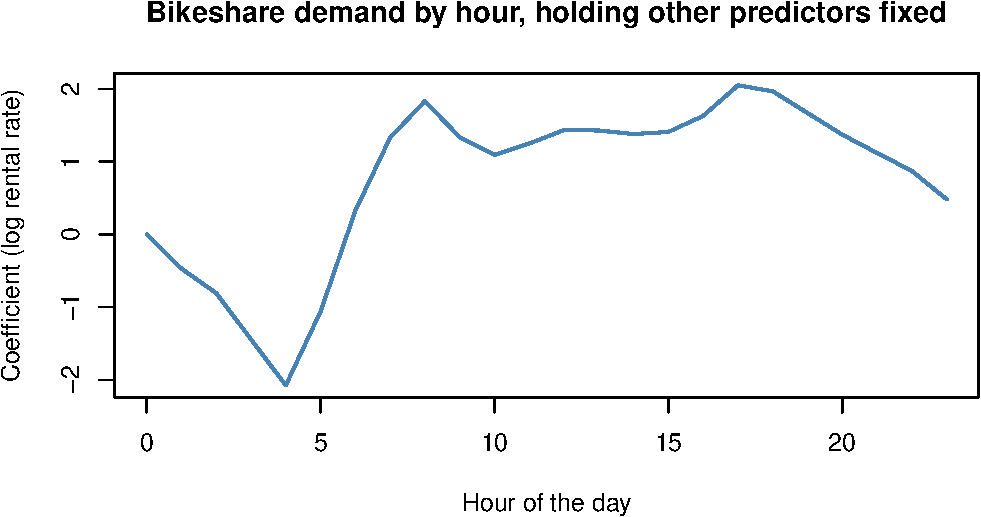
\includegraphics{ch04_lab_files/figure-latex/poisson-hourly-1} \end{center}

The hourly coefficients trace out the expected daily commuting rhythm
--- sharp peaks around the morning and evening rush hours, with a trough
overnight --- which a positive-count model like this one can represent
naturally, in a way a plain linear regression fit to the raw counts
would not.

\end{document}
